% ----------------------------------------------------------------------
%  Pracovní úkoly
% ----------------------------------------------------------------------
\section{Pracovní úkoly}

\begin{enumerate}
\item Při zapnutém kompresoru proměřte časovou závislost teplot v obou rezervoárech. Současně zaznamenávejte elektrický příkon kompresoru a časovou závislost tlaků v aparatuře. Graficky znázorněte.

\item Vyhodnoťte chladicí a topný faktor zdroje tepla, graficky znázorněte závislosti ε = ε(ΔT) a τ = τ(ΔT)

\item Při vypnutém kompresoru proměřte časovou závislost teploty vody v obou rezervoárech. Graficky znázorněte a závislost fitujte exponenciálou. Diskutujte koeficienty naměřené závislosti.

\item Ze změny teploty rezervoáru po vypnutí kompresoru určete dolní odhad tepelných ztrát.

\end{enumerate}

% ----------------------------------------------------------------------
%  Teoretická část
% ----------------------------------------------------------------------
\section{Teoretická část}

Podstatou fungování tepelného čerpadla je předávání tepla z jednoho rezervoáru do druhého. Používají se různá média pro přenos tepla, v našem případě je v rezervoárech umístěna destilovaná voda, kde rezervoár, který se během fungování otepluje je označen červeně a druhý, který se ochlazuje má modrou barvu.

Tepelné čerpadlo je tvořeno uzavřeným okruhem, kde koluje pracovní látka 1,1,1,2-
tetrafluorethan. V oblasti modrého kolektoru se v měděném potrubí chladivo nachází v plynné fázi. Odtud je přečerpáváno do kompresoru, kde je zvyšován tlak a tím dochází ke zkapalnění. Zde začíná vysokotlaká část čerpadla. Během tohoto procesu látka odevzdává část energie do červeného kolektoru, což způsobuje zvyšování teploty vody uvnitř kolektoru. Odtud putuje chladivo v kapalném stavu přes vysokotlaký manometr do kolektoru. Zde se látka hromadí a je regulovaně propouštěna do expanzního ventilu. Zde je snižován tlak a kapalina se tím vypařuje. Začíná tak nízkotlaká část čerpadla. Tím odebírá teplo z okolí a snižuje teplotu modrého rezervoáru. Je zde také umístěn nízkotlaký barometr. Následuje teplotní čidlo, které reguluje expanzní ventil proto, aby se do kompresoru dostávala pouze plynná fáze. Za čidlem se nachází již kompresor, který takto celý okruh uzavírá, jak je znázorněno na obrázku \ref{fig:tepelne-cerpadlo}.

\begin{figure}[h]
    \centering
    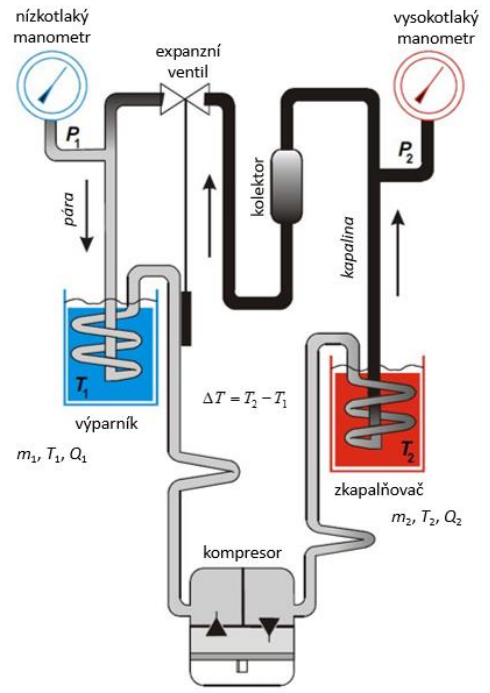
\includegraphics[width=0.4\linewidth]{27 - Tepelné čerpadlo//Protokol_tepelné čerpadlo//img/Schéma tepelného čerpadla.png}
    \caption{Schéma tepelného čerpadla}
    \label{fig:tepelne-cerpadlo}
\end{figure}

\newpage

Teplota v různých místech okruhu je snímána digitálním termometrem s výstupem do počítače. Teplota T1 je měřena v modrém rezervoáru a T2 v červeném. Uvnitř kbelíků jsou umístěna míchadla, díky kterým je teplota vody ve všech místech podobná. Dále je teplota T3 odečítána ze vzduchu v okolí a nakonec teplota T4 na povrchu kompresoru.

U ideálního tepelného čerpadla by platila rovnice zákonu zachování energie

\begin{equation}
    \Delta Q_1 + W = \Delta Q_2
\end{equation}

kde \(\Delta Q_1\) je odebrané teplo, \(W\) energie dodaná elektrickým proudem a \(\Delta Q_2\) teplo, které přijme červený rezervoár. Práce, kterou tepelný stroj vykonává, je rovna

\begin{equation}
    W = P \cdot \Delta t
\end{equation}

kde P je průměrný výkon za čas t. Dodané, popř. odevzdané teplo lze vyjádřit jako

\begin{equation}
    \Delta Q_{1,2} = m_{1,2} c \Delta T_{1,2}
\end{equation}

kde \(m_{1,2}\) je hmotnost vody v rezervoáru, \(c\) měrné teplo vody a \(\Delta T_{1,2}\) rozdíl teplot v daném rezervoáru. V reálném případě však do vztahu (1) vstupují tepelné ztráty \(\Delta Q\).

Abychom mohli určit kvalitu daného tepelného čerpadla a porovnat ho s jinými zavádí se tzv. chladící faktor zdroje chladu, který je definován jako

\begin{equation}
    \varepsilon (\Delta T) = \frac{\Delta Q_1}{P \Delta t} = \frac{c m_1 \Delta T_1}{P \Delta t}
\end{equation}

Analogicky můžeme popsat topnou účinnost pomocí topného faktoru zdroje tepla

\begin{equation}
    \tau (\Delta t) = \frac{c m_2 \Delta T_2}{P \Delta t}
\end{equation}

% ----------------------------------------------------------------------
%  Výsledky a zpracování měření
% ----------------------------------------------------------------------
\section{Výsledky a zpracování měření}

\subsection{Laboratorní podmínky}

    Měření bylo prováděno za laboratorních podmínek uvedených v tabulce \ref{tab:laboratorni-podminky}.

    \begin{table}[h]
        \centering
        \begin{tabular}{|c|c|c|} 
        \hline
            t / °C & p / hPa & vlhkost / \%RH  \\ 
        \hline
            23,9(4)   & 981(2)   & 38,8(25)            \\
        \hline
        \end{tabular}
        \caption{Laboratorní podmínky}
        \label{tab:laboratorni-podminky}
    \end{table}

\subsection{Zapnutý kompresor}

Při zapnutém kompresoru byly v minutovém intervalu zapisovány teploty T1 - T4, tlak v nízkotlaké a vysokotlaké části a příkon dodávaný kompresoru. Závislosti teploty v modrém a červeném rezervoáru na čase jsou znázorněn na obrázku \ref{fig:T1(t),T2(t)}. Dále je na obrázku \ref{fig:P(t)} zobrazena závislost obou tlaků na čase. Nakonec na obrázku \ref{fig:P0(t)} je naměřena závislost příkonu na čase.

\newpage

\begin{figure}[h]
    \centering
    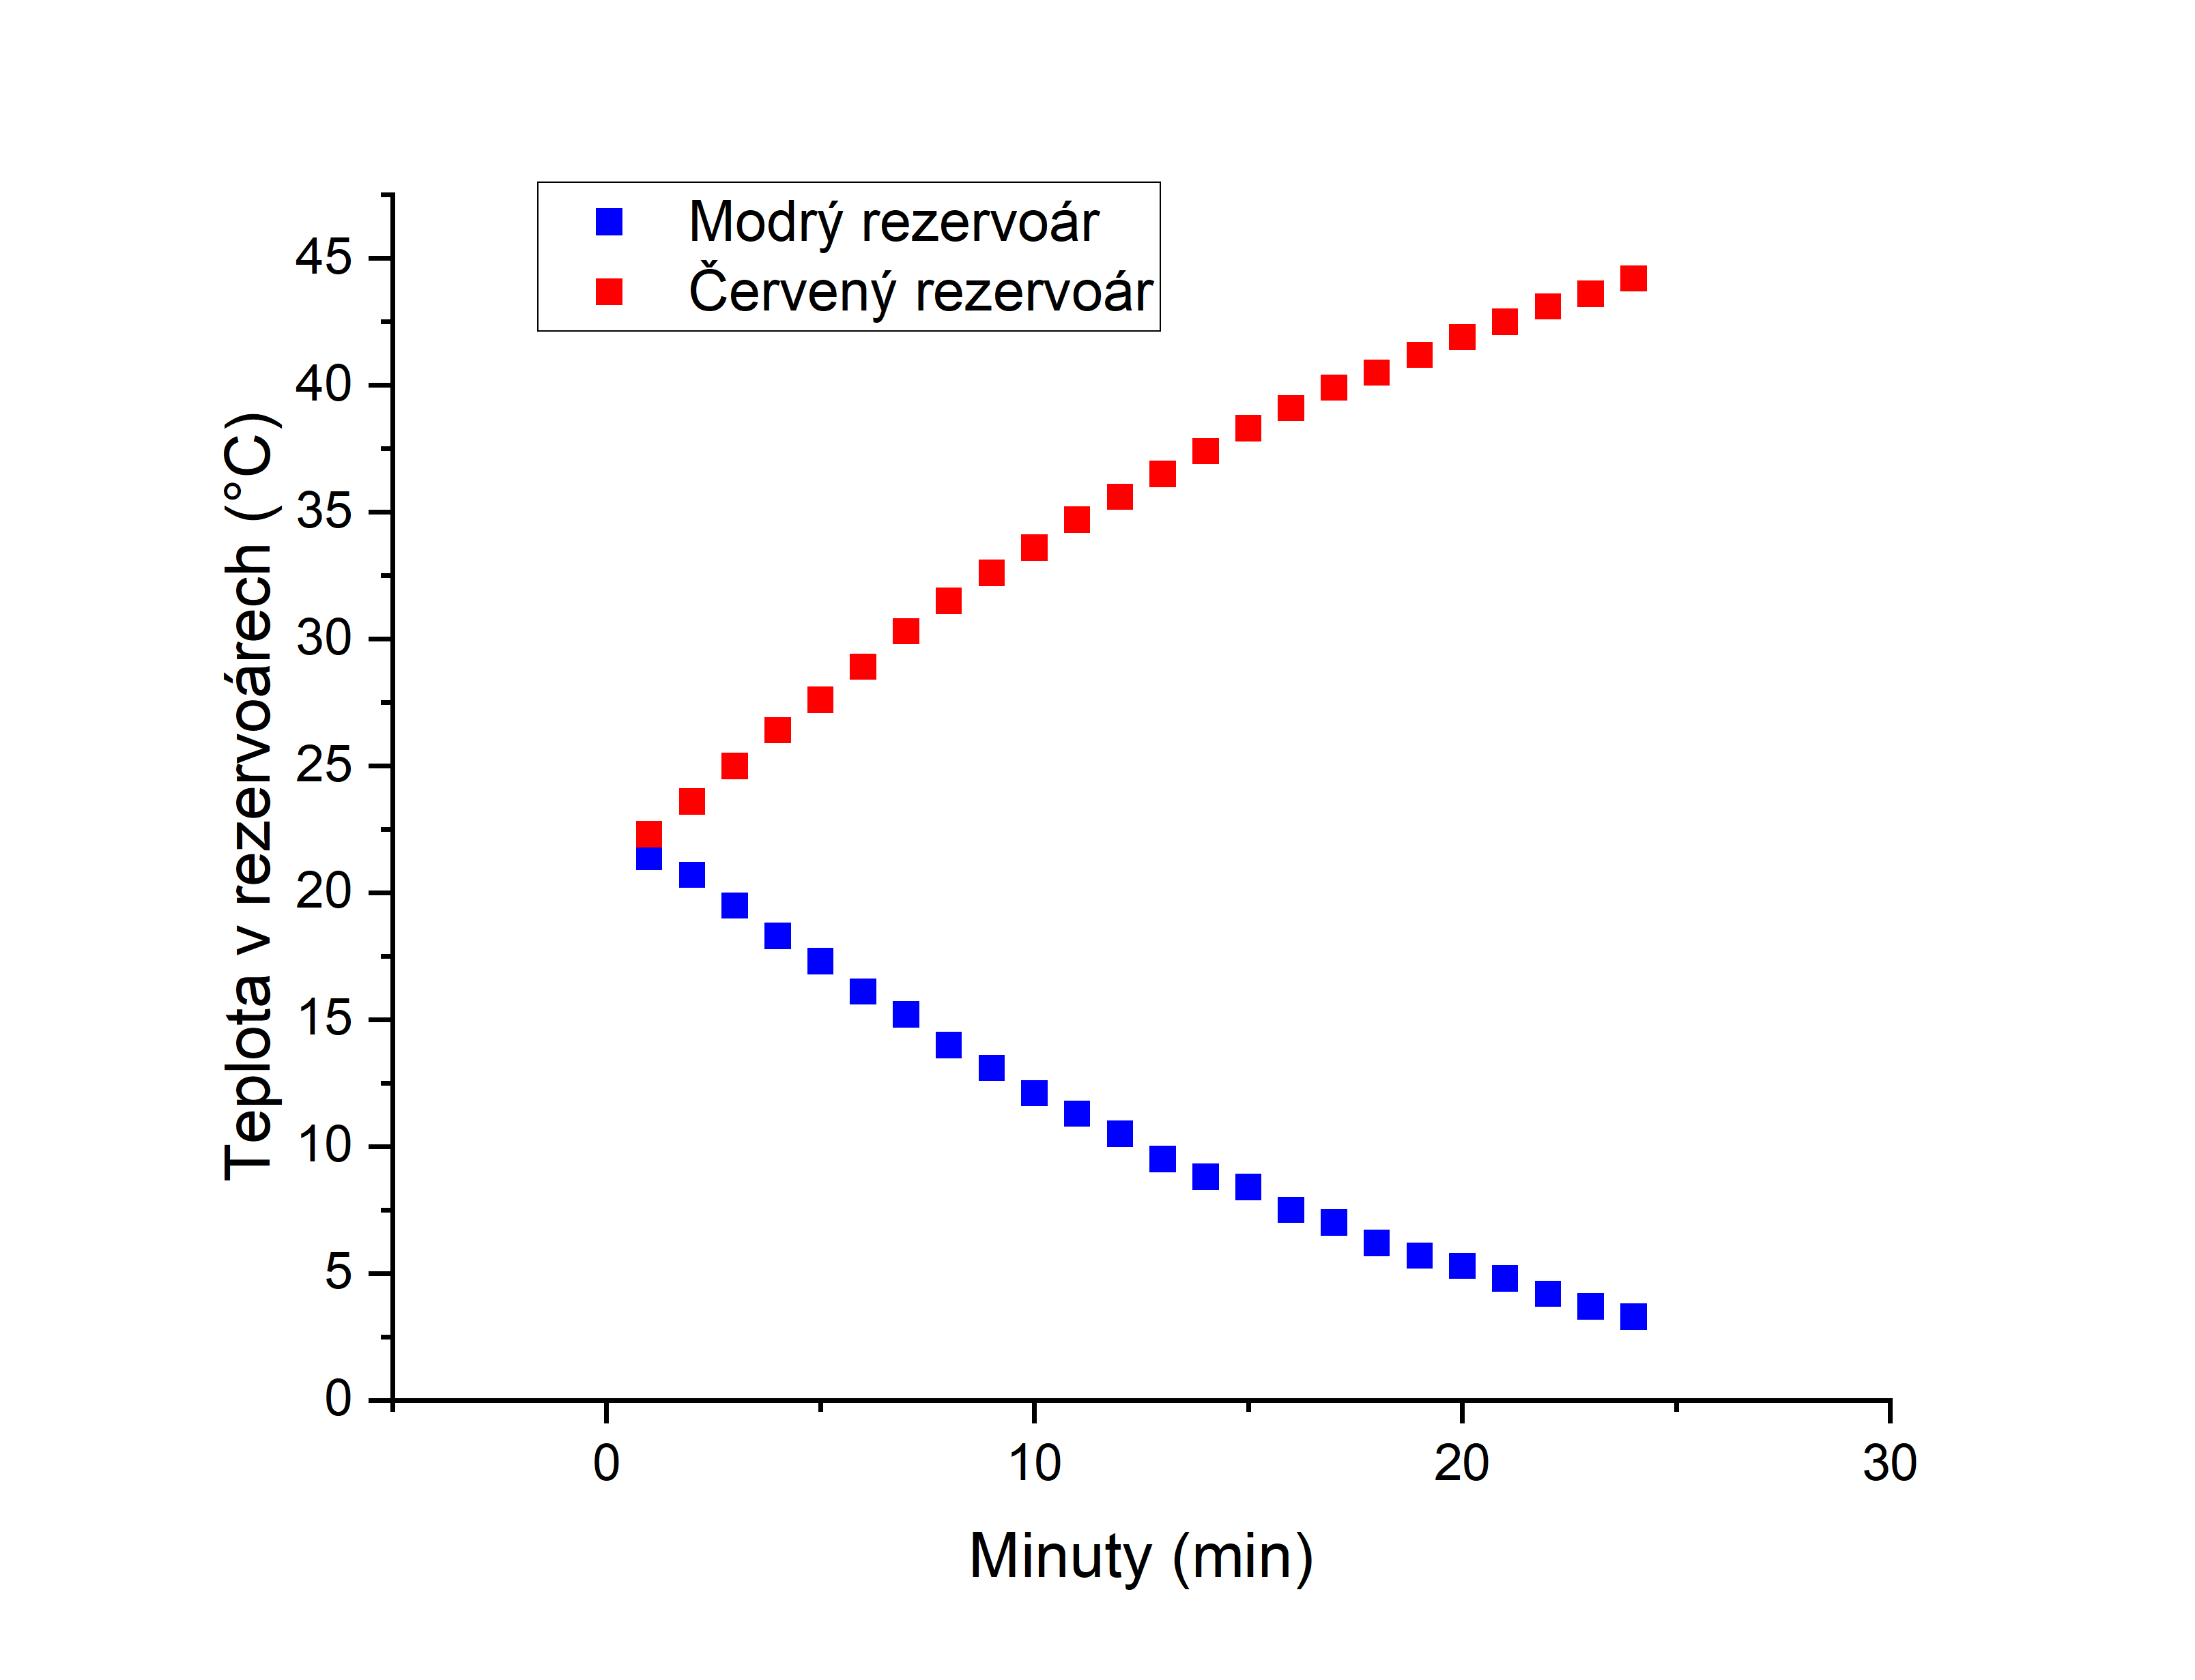
\includegraphics[width=0.68\linewidth]{27 - Tepelné čerpadlo//Protokol_tepelné čerpadlo//img/T1(t), T2(t) zap.png}
    \caption{Závislost teploty T1 a T2 na čase}
    \label{fig:T1(t),T2(t)}
\end{figure}

\begin{figure}[h]
    \centering
    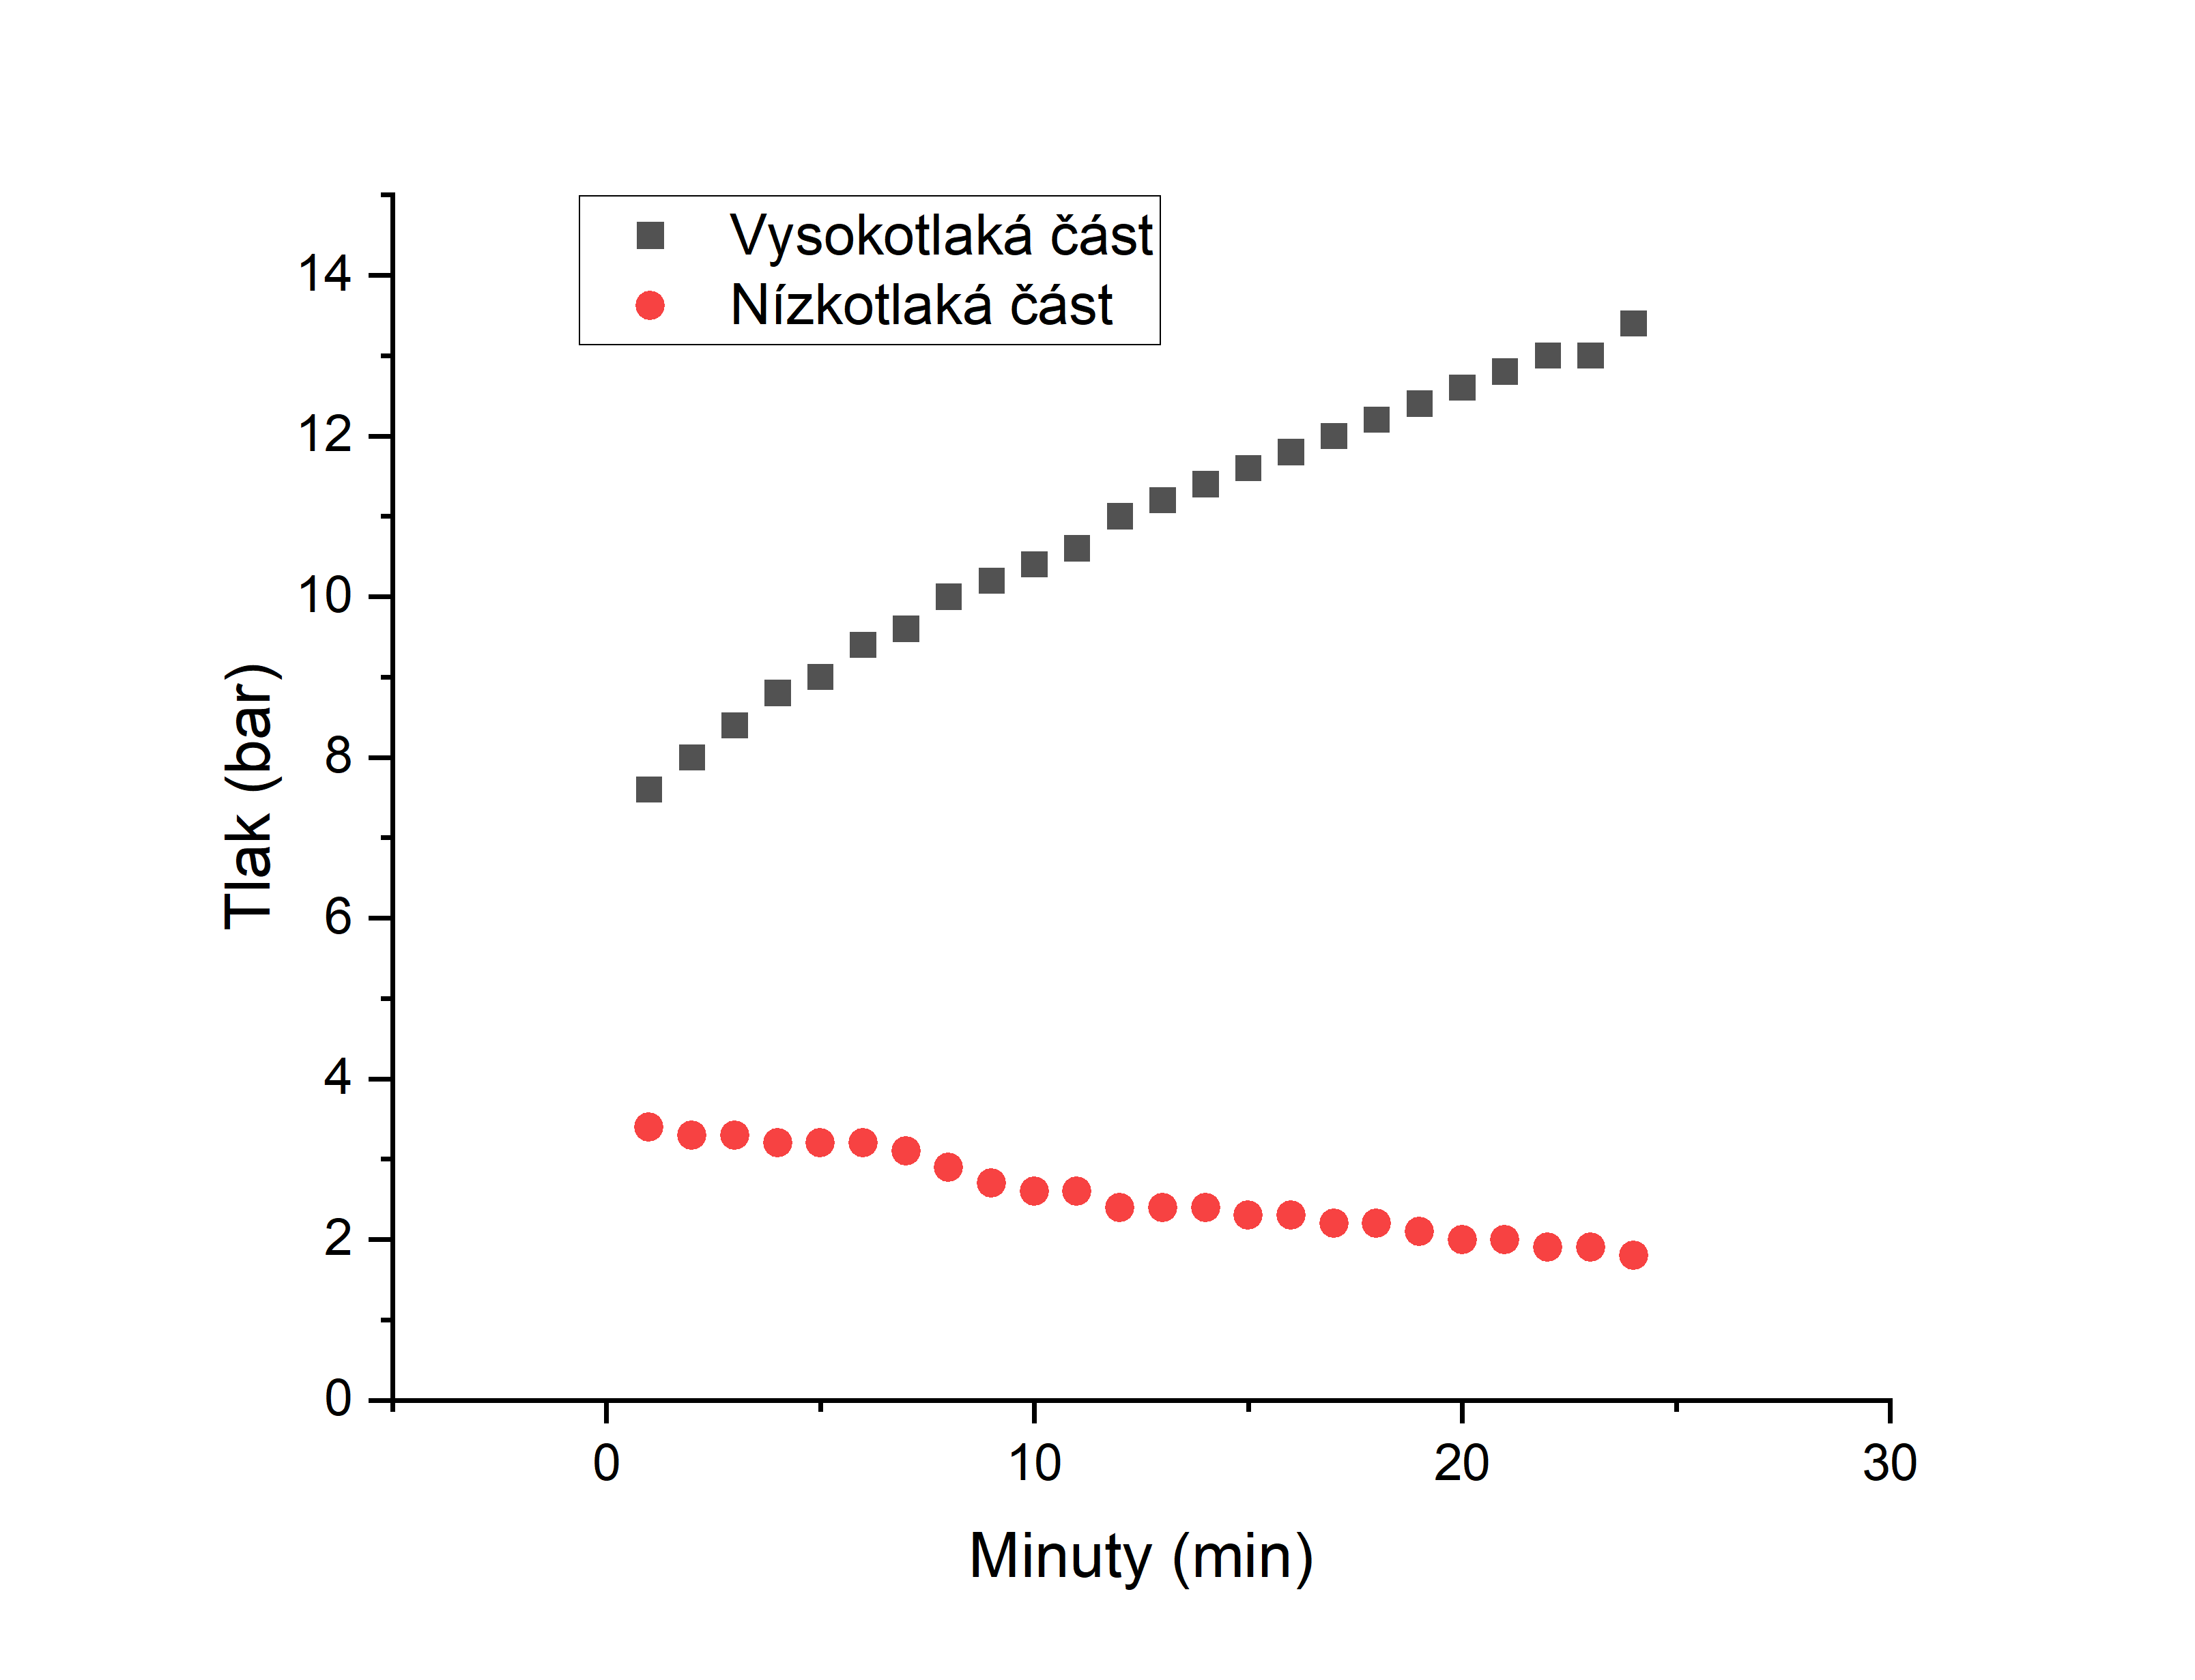
\includegraphics[width=0.68\linewidth]{27 - Tepelné čerpadlo//Protokol_tepelné čerpadlo//img/P(t) zap.png}
    \caption{Závislost tlaků na čase}
    \label{fig:P(t)}
\end{figure}

\newpage

\begin{figure}[h]
    \centering
    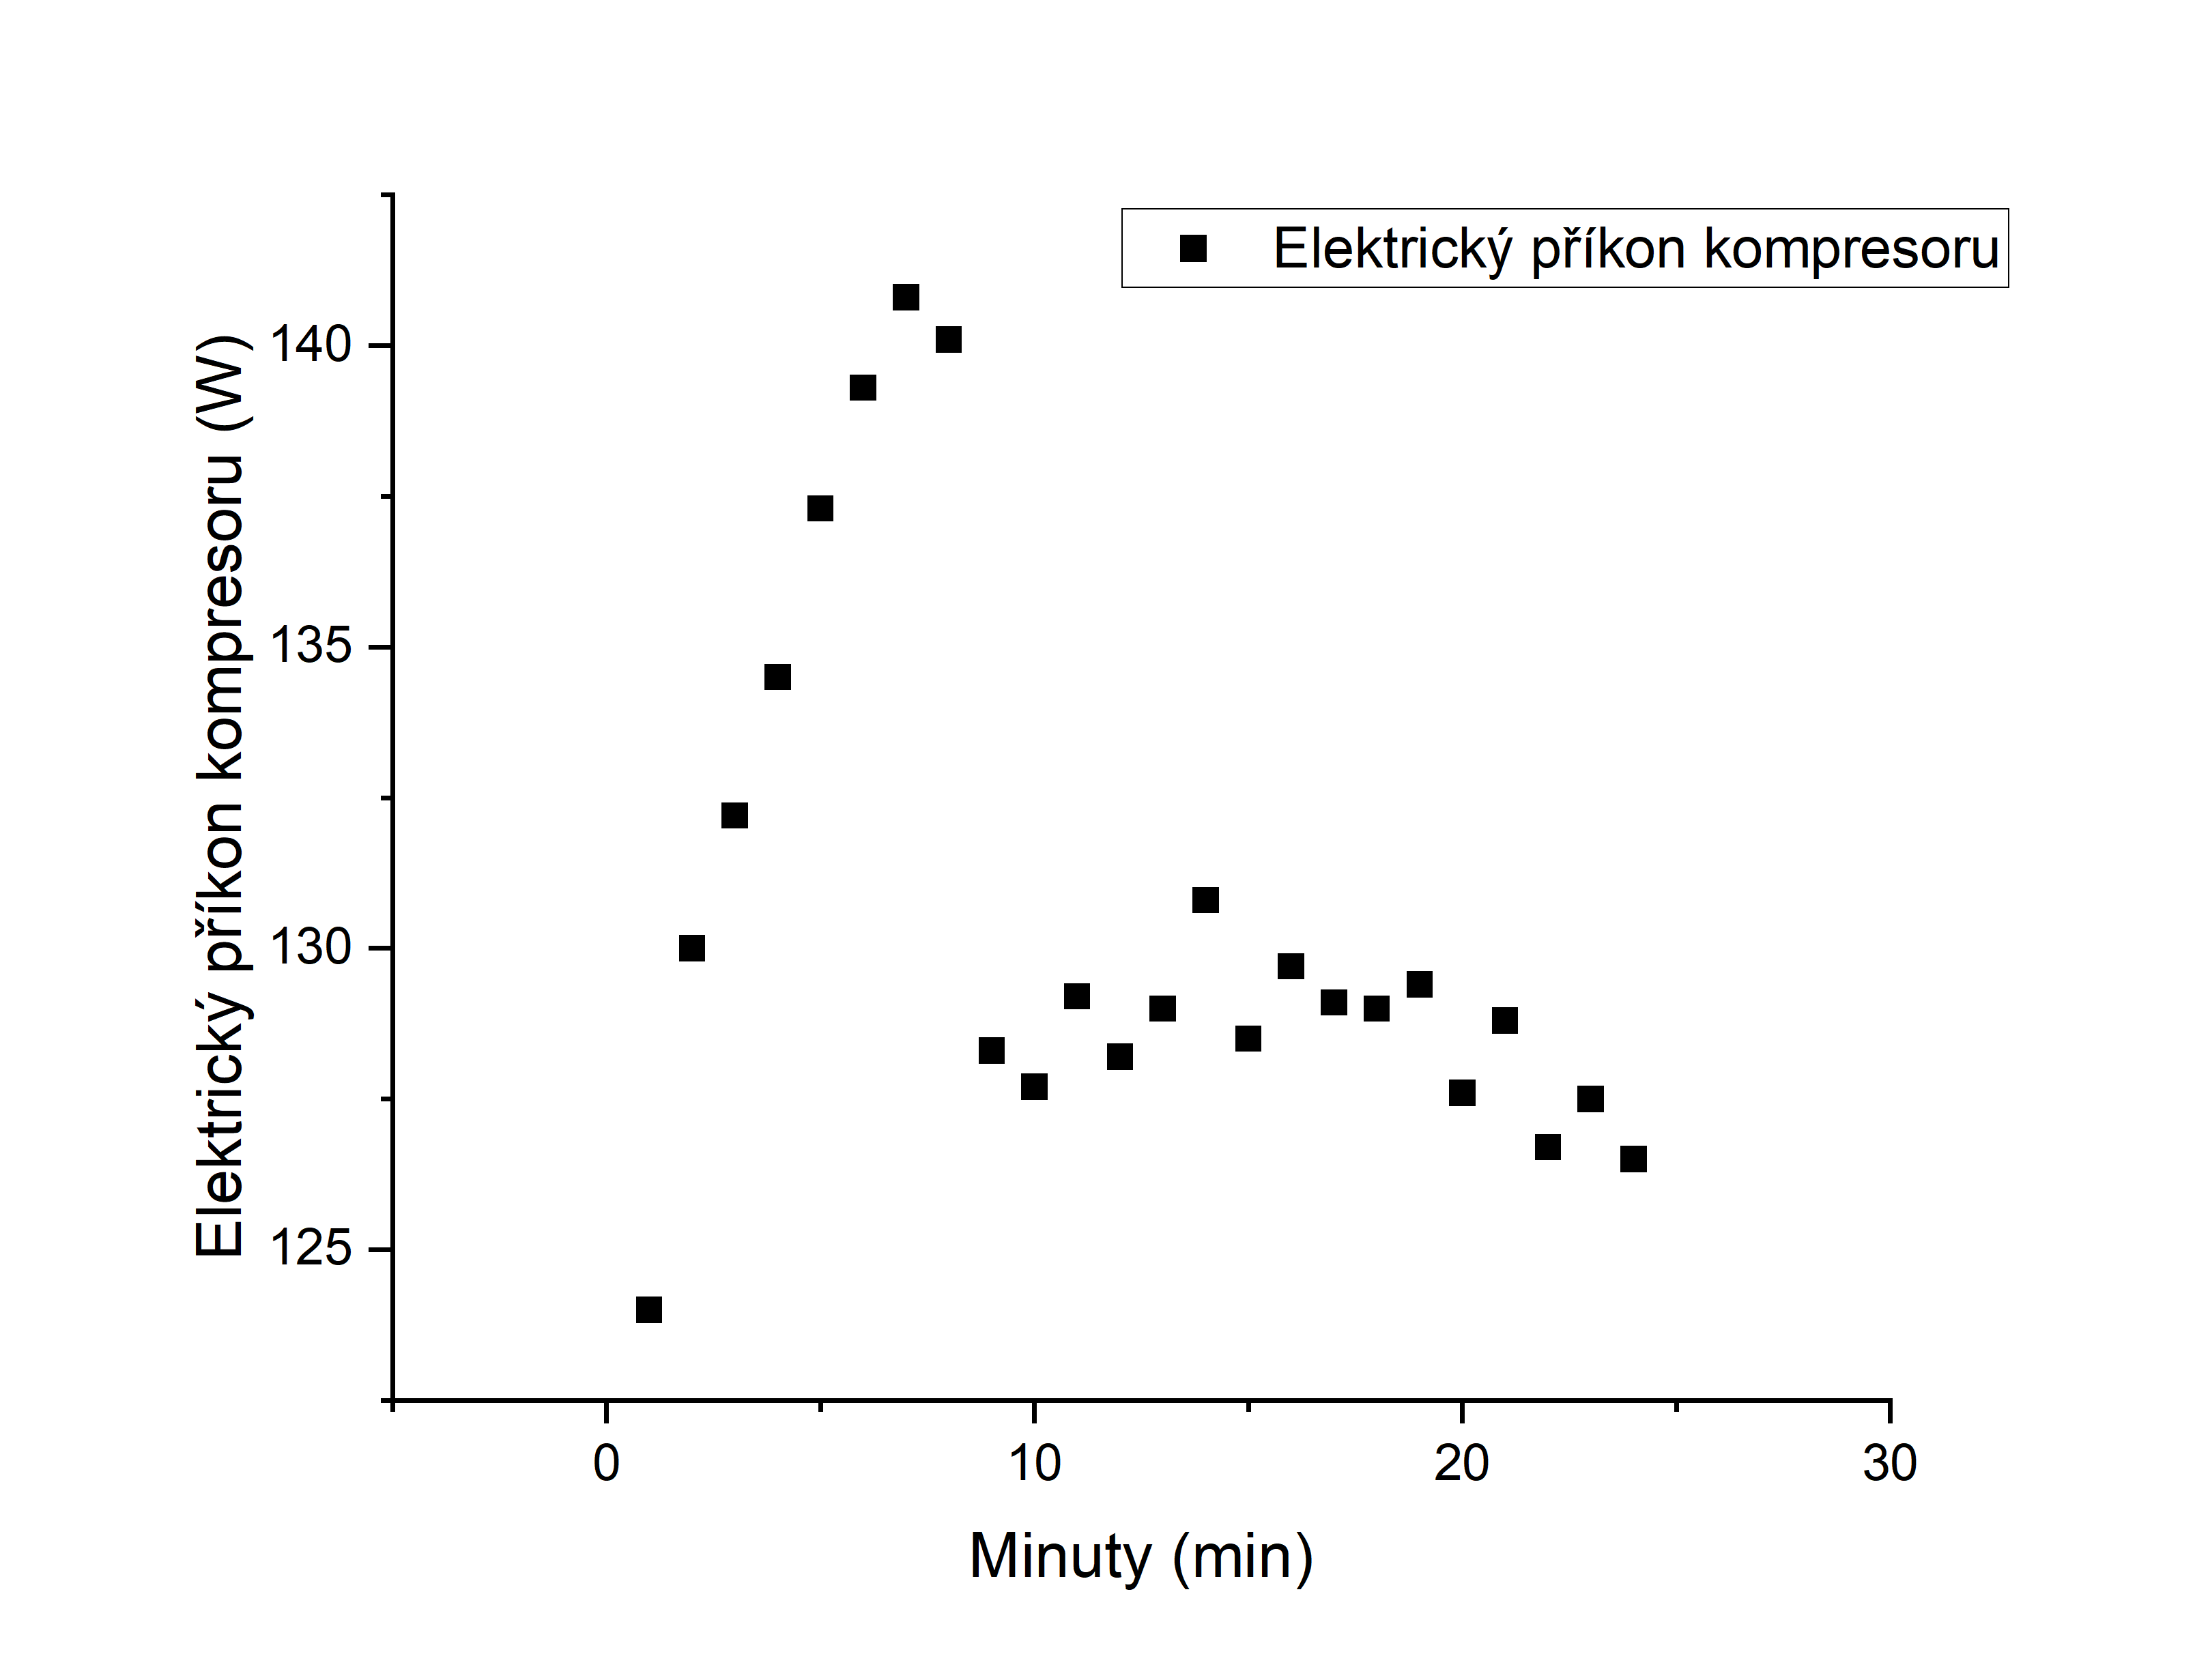
\includegraphics[width=0.68\linewidth]{27 - Tepelné čerpadlo//Protokol_tepelné čerpadlo//img/P0(t).png}
    \caption{Závislost příkonu na čase}
    \label{fig:P0(t)}
\end{figure}

Pro výpočet chladícího faktoru použijeme vztah (4). Pro výpočty budeme používat hodnoty uvedené v tabulce \ref{tab:hodnoty}.

\begin{table}[h]
\centering
\begin{tabular}{|c|c|} 
\hline
Měrné teplo vody       & 4180 J/kg\cdot K   \\ 
\hline
Hustota vody při 24 °C & 997 kg \cdot m^{-3}    \\ 
\hline
Hmotnost m_1          & 4 kg      \\ 
\hline
Hmotnost m_2          & 4 kg      \\ 
\hline
Průměrný příkon        & 130,6 W  \\ 
\hline
\Delta T_1                   & 18,1 K  \\ 
\hline
\Delta T_2                   & 21,9 K  \\ 
\hline
\Delta t                      & 1380 s   \\
\hline
\end{tabular}
\caption{Použité hodnoty}
\label{tab:hodnoty}
\end{table}

Odtud získáme chladící faktor

\begin{equation}
    \nonumber
    \varepsilon = 1,67
\end{equation}

a topný faktor

\begin{equation}
    \nonumber
    \tau = 2,03
\end{equation}

Na obrázku \ref{fig:teploty-cas-zap} jsou zobrazeny závislosti teplot T1 - T4 na čase. Tento graf je exportovaný přímo z programu používaném pro sběr dat z termometru. Oproti předchozím grafů navíc porovnává teplotu T3 okolí čerpadla a T4 na povrchu kompresoru.

\newpage

\begin{figure}[h]
    \centering
    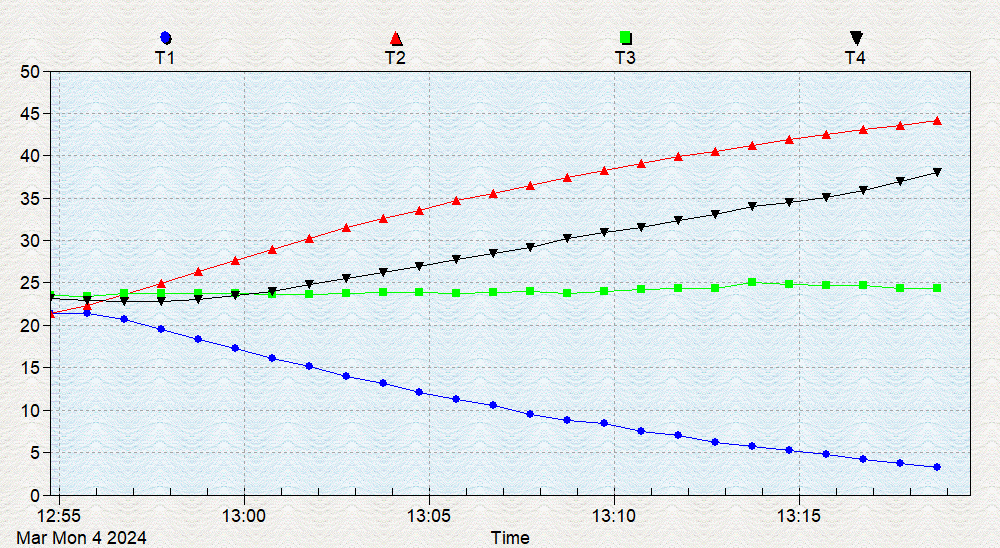
\includegraphics[width=0.8\linewidth]{27 - Tepelné čerpadlo//Protokol_tepelné čerpadlo//img/Zap.png}
    \caption{Závislost teplot na čase}
    \label{fig:teploty-cas-zap}
\end{figure}

\subsection{Vypnutý kompresor}

Jakmile tepelné čerpadlo dosáhlo požadovaného rozdílu teplot mezi rezervoáry, kompresor byl odpojen od elektrického proudu a byla sledována změna teplot T1 - T4 a tlaků obou částí čerpadla. Na grafu \ref{fig:T1(t),T2(t)-vyp} je průběh závislosti teplot obou rezervoárů na čase, který je fitovaný exponenciálou.

\begin{figure}[h]
    \centering
    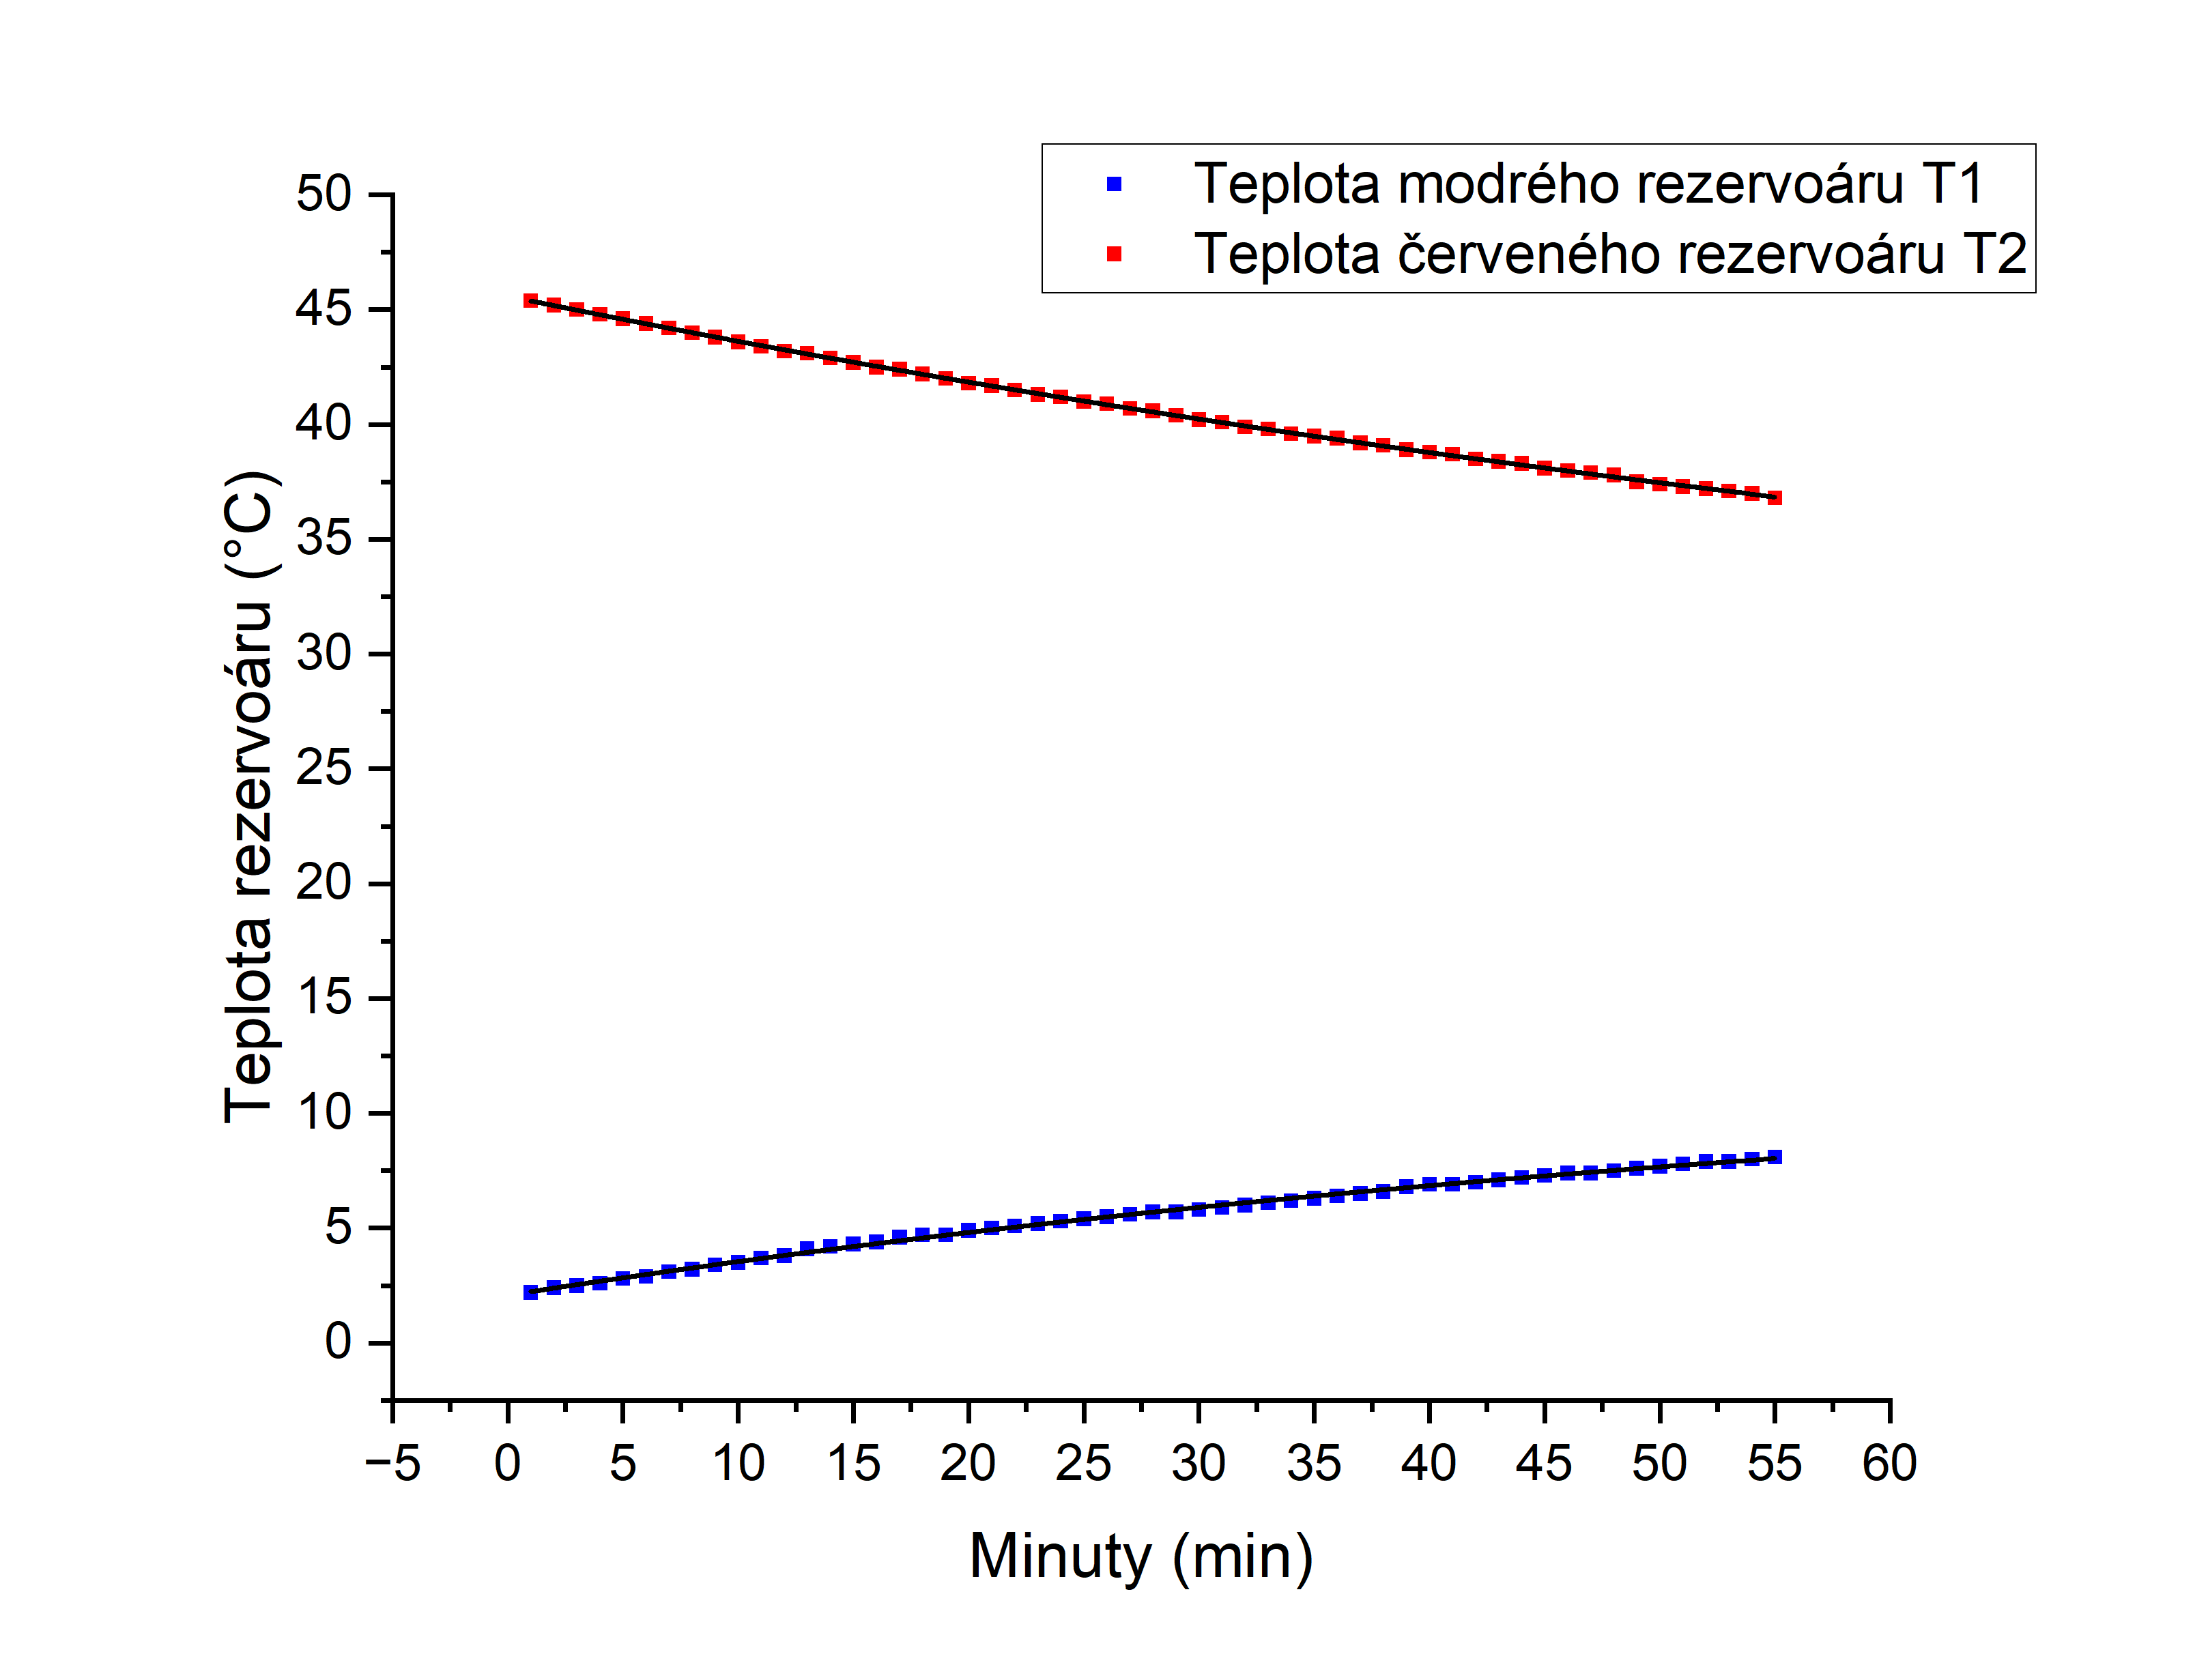
\includegraphics[width=0.68\linewidth]{27 - Tepelné čerpadlo//Protokol_tepelné čerpadlo//img/T1(t), T2(t) vyp.png}
    \caption{Závislost teploty T1 a T2 na čase}
    \label{fig:T1(t),T2(t)-vyp}
\end{figure}

Exponenciála je daná rovnicí

\begin{equation}
    \nonumber
    y = y_0 + A \cdot e^{R_0 \cdot x}
\end{equation}

Exponenciální křivky modrého a červeného rezervoáru mají následující koeficienty

\begin{equation}
    \nonumber
    y_{červená} = 24,9 + 20,7 \cdot e^{-0,01 x}
\end{equation}

\begin{equation}
    \nonumber
    y_{modrá} = 12,8 - 10,6 \cdot e^{-0,01 x}
\end{equation}

Na grafu \ref{fig:P(t)-vyp} je zobrazena závislost tlaků na čase při vypnutém kompresoru.

\begin{figure}[h]
    \centering
    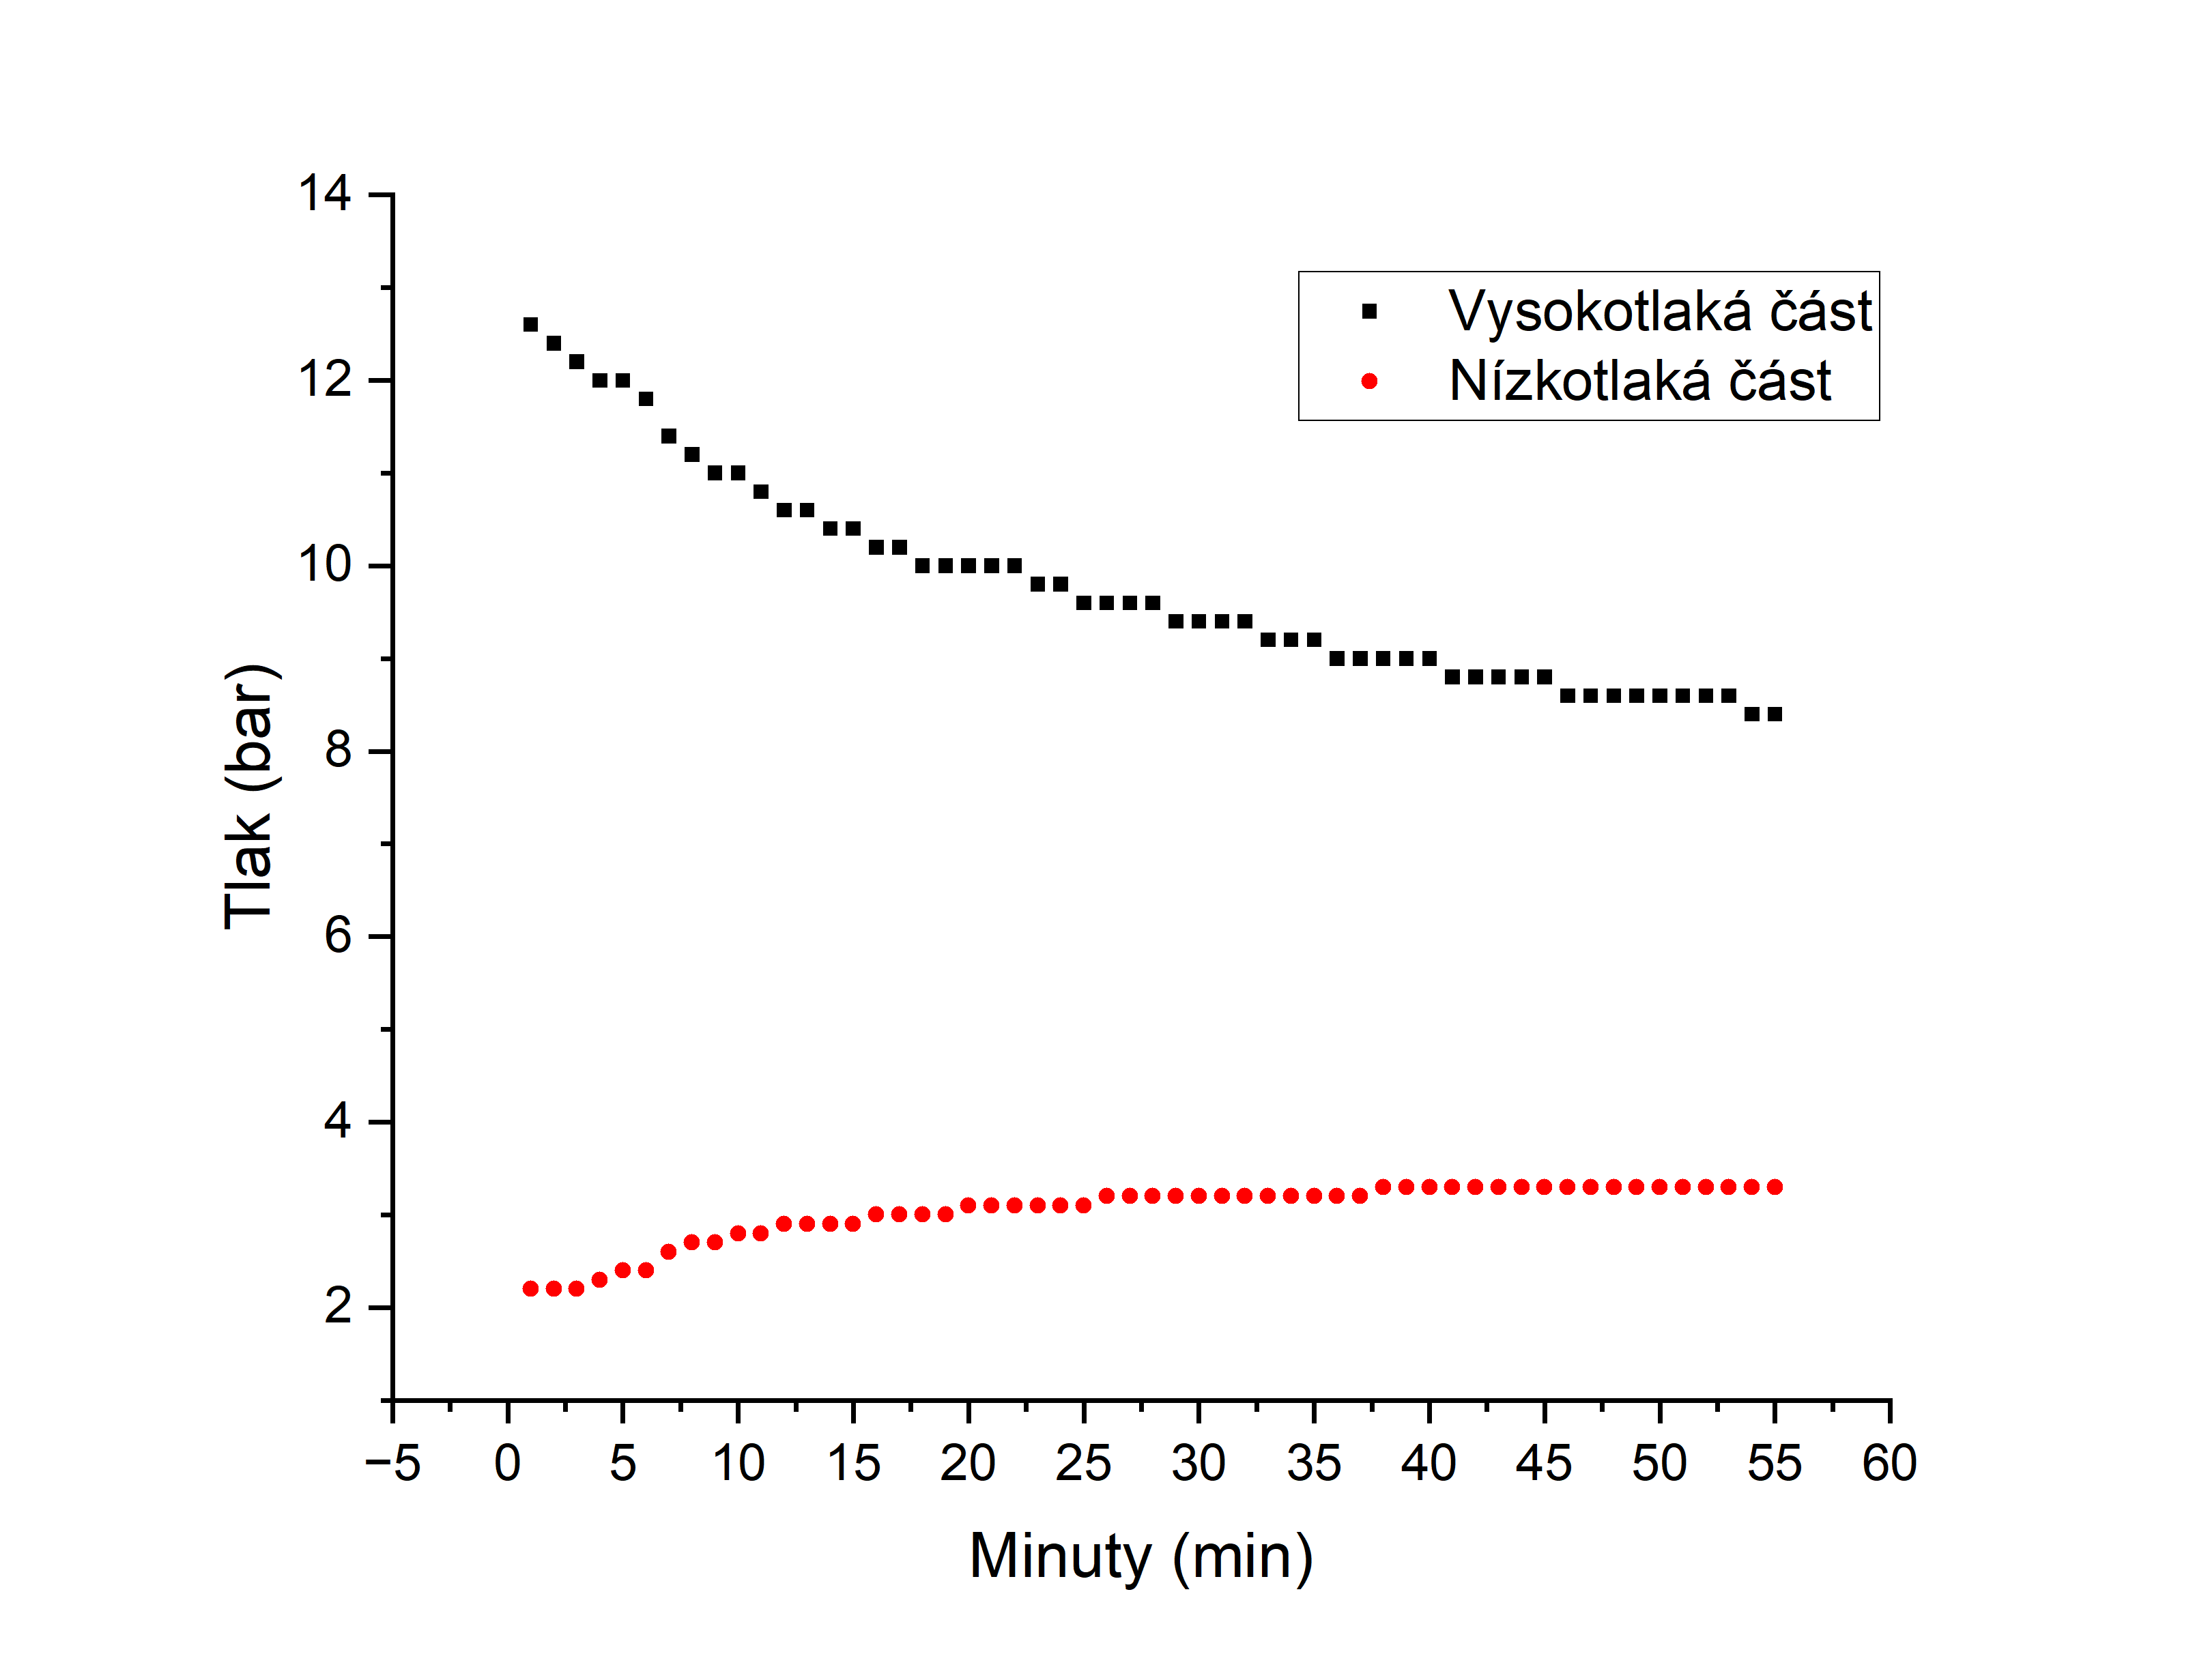
\includegraphics[width=0.68\linewidth]{27 - Tepelné čerpadlo//Protokol_tepelné čerpadlo//img/P(t) vyp.png}
    \caption{Závislost tlaků na čase}
    \label{fig:P(t)-vyp}
\end{figure}

Na obrázku \ref{fig:T(t)-vyp} jsou opět vidět všechny čtyři teploty přímo z termometru

\begin{figure}[h]
    \centering
    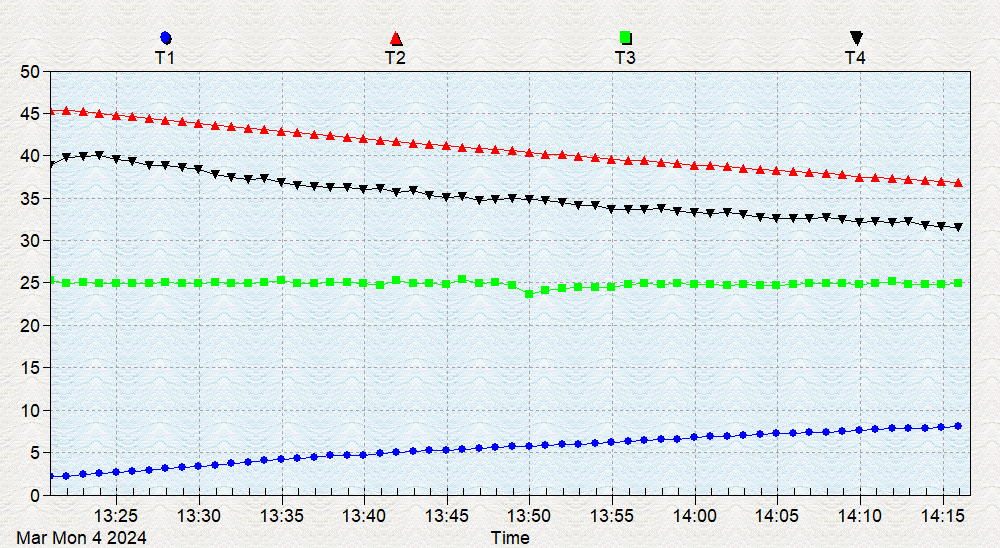
\includegraphics[width=0.8\linewidth]{27 - Tepelné čerpadlo//Protokol_tepelné čerpadlo//img/Vyp.png}
    \caption{Závislost teplot na čase}
    \label{fig:T(t)-vyp}
\end{figure}

\subsection{Tepelné ztráty}

Podle (2) je práce, kterou čerpadlo vykoná, rovna

\begin{equation}
    \nonumber
    W = 188,06 \; kJ
\end{equation}

Podle (3) je odebrané a dodané teplo rovno

\begin{equation}
    \nonumber
    \Delta Q_1 = 4,87 \; MJ
\end{equation}

\begin{equation}
    \nonumber
    \Delta Q_2 = 4,93 \; MJ
\end{equation}

Celkové tepelné ztráty se vypočítají jako

\begin{equation}
    \Delta Q = \Delta Q_1 + W - \Delta Q_2
\end{equation}

Odtud

\begin{equation}
    \Delta Q = 124,5 \; kJ
\end{equation}


% ----------------------------------------------------------------------
%  Diskuse výsledků
% ----------------------------------------------------------------------			
\section{Diskuse výsledků}

% ----------------------------------------------------------------------
%  Závěr
% ----------------------------------------------------------------------
\section{Závěr}
